%texexptitled======================================================================
% lab1-gcd
%-----------------------------------------------------------------------
%

\documentclass[11pt]{article}

% Package includes

\usepackage{graphicx}
\usepackage{color}
\usepackage{comment}
\usepackage{multirow}
\usepackage{askmaps}
\usepackage{amssymb}
\usepackage{amsmath}
\usepackage{tikz}
\usepackage{circuitikzgit}
\usetikzlibrary{arrows, positioning, shapes.geometric, circuits.logic.US}
\tikzstyle{line}=[draw]
\tikzstyle{arrow}=[draw, -latex]

% Wrap long URLs with hyphens
\PassOptionsToPackage{hyphens}{url}\usepackage{hyperref}
\usepackage{pdftexcmds}
\usepackage{upquote}
\usepackage{textcomp}
\usepackage{minted}
\usepackage[listings]{tcolorbox}
\usepackage{enumerate}
\usepackage{enumitem}
\usepackage{mathtools}
\DeclarePairedDelimiter{\ceil}{\Big\lceil}{\Big\rceil}

\tcbset{
texexp/.style={colframe=black, colback=lightgray!15,
         coltitle=white,
         fonttitle=\small\sffamily\bfseries, fontupper=\small, fontlower=\small},
     example/.style 2 args={texexp,
title={Question \thetcbcounter: #1},label={#2}},
}

\newtcolorbox{texexp}[1]{texexp}
\newtcolorbox[auto counter]{texexptitled}[3][]{%
example={#2}{#3},#1}

\setlength{\topmargin}{-0.5in}
\setlength{\textheight}{9in}
\setlength{\oddsidemargin}{0in}
\setlength{\evensidemargin}{0in}
\setlength{\textwidth}{6.5in}

% Useful macros

\newcommand{\note}[1]{{\bf [ NOTE: #1 ]}}
\newcommand{\fixme}[1]{{\bf [ FIXME: #1 ]}}
\newcommand{\wunits}[2]{\mbox{#1\,#2}}
\newcommand{\um}{\mbox{$\mu$m}}
\newcommand{\xum}[1]{\wunits{#1}{\um}}
\newcommand{\by}[2]{\mbox{#1$\times$#2}}
\newcommand{\byby}[3]{\mbox{#1$\times$#2$\times$#3}}


\newenvironment{tightlist}
{\begin{itemize}
 \setlength{\parsep}{0pt}
 \setlength{\itemsep}{-2pt}}
{\end{itemize}}

\newenvironment{titledtightlist}[1]
{\noindent
 ~~\textbf{#1}
 \begin{itemize}
 \setlength{\parsep}{0pt}
 \setlength{\itemsep}{-2pt}}
{\end{itemize}}

% Change spacing before and after section headers

\makeatletter
\renewcommand{\section}
{\@startsection {section}{1}{0pt}
 {-2ex}
 {1ex}
 {\bfseries\Large}}
\makeatother

\makeatletter
\renewcommand{\subsection}
{\@startsection {subsection}{1}{0pt}
 {-1ex}
 {0.5ex}
 {\bfseries\normalsize}}
\makeatother

% Reduce likelihood of a single line at the top/bottom of page

\clubpenalty=2000
\widowpenalty=2000

% Other commands and parameters

\pagestyle{myheadings}
\setlength{\parindent}{0in}
\setlength{\parskip}{10pt}

% Commands for register format figures.

\newcommand{\instbit}[1]{\mbox{\scriptsize #1}}
\newcommand{\instbitrange}[2]{\instbit{#1} \hfill \instbit{#2}}

\newif\ifsolution

\if\issolution1
\newenvironment{solution}
    {\color{red}}
    {\color{black}}
\solutiontrue
\else
\excludecomment{solution}
\solutionfalse
\fi


\graphicspath{{./figs/}}


%-----------------------------------------------------------------------
% Document
%-----------------------------------------------------------------------

\begin{document}
\def\PYZsq{\textquotesingle}


\newcommand{\headertext}{EE142 Problem Set 9}
\renewcommand{\thesubsection}{\thesection.\alph{subsection}}

\title{\vspace{-0.4in}\Large \bf \headertext \vspace{-0.1in}}
\author{Vighnesh Iyer}

\date{\today}
\maketitle

\markboth{\headertext}{\headertext}
\thispagestyle{empty}

\section{Review of Important Concepts}
{\color{blue} Assume a memoryless distortion circuit is modeled by
$I_{out} = a_0 + a_1 V_{in} + a_2 V_{in}^2 + a_3 V_{in}^3$ and the input DC bias voltage is $V_{in,0}$.}

\begin{enumerate}[label=(\alph*)]
    \item {\color{blue} Derive IIP3, OIP3, $IP_{1dB}$, and $IP_{3dB}$}

    \item {\color{blue} If IIP3 is 10V, what is the input-blocker level that degrades the small-signal gain of the desired signal by 2dB?}

    \item {\color{blue} Following part (b), what will be the tolerable blocker levels for a two-tone blocker?}

    \item {\color{blue} If IIP3 is 10V, what are the $IP_{1dB}$ for two-tone and three-tone inpnut signals?}

    \item {\color{blue} If the modeled circuit is a BJT with $I_{out} = I_s \exp(V_{be}/V_{T})$, use a math tool to find the actual output third-harmonic current as a function of the input magnitude. Compare the actual values to the estimated values via the power series.}
\end{enumerate}

\section{Distortion of a Source Follower}
{\color{blue} For the source follower shown below, calculate the required bias current ($I_{bias}$ and W/L for the long-channel transistor to drive the load with a swing of 100 mV (at both $f_1$ and $f_2$), with IM3 equal to -50 dBc.}

{\color{red} Correction: vout= 0.1cos(2pi*f1*t)+0.1cos(2pi*f2*t) vin magnitude is not specified}

\begin{figure}[H]
    \centering 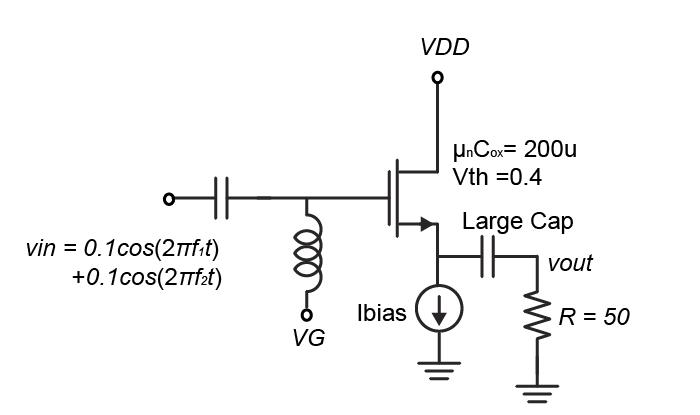
\includegraphics[width=0.8\textwidth]{problem2_schematic.jpg}
\end{figure}

\section{Pre-distortion and Source-degeneration Linearizer}
\begin{figure}[H]
    \centering 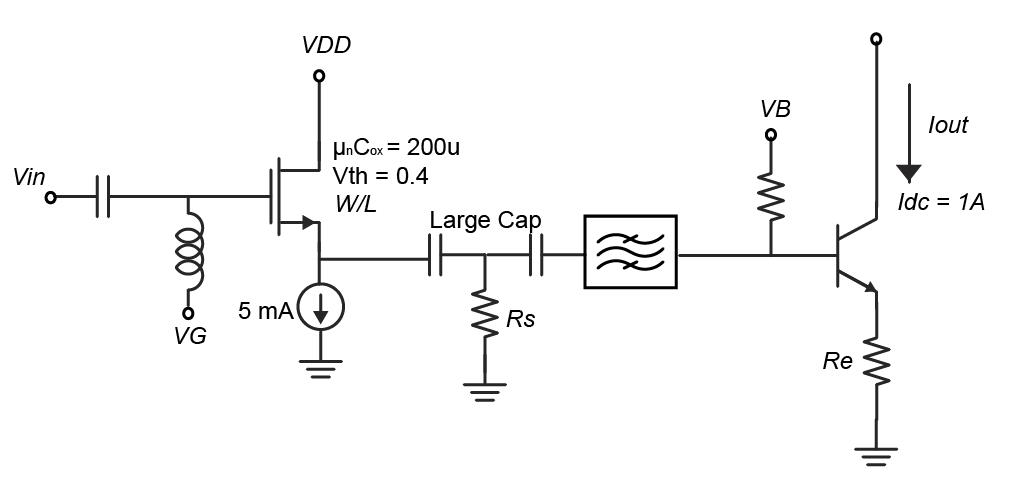
\includegraphics[width=\textwidth]{problem3_schematic.jpg}
\end{figure}

\begin{enumerate}[label=(\alph*)]
    \item {\color{blue} For the above schematic, what are the OIP3 of the BJT stage for $R_e = 0 \Omega$ and $R_e = 0.02 \Omega$?}

    \item {\color{blue} What are the two possible $R_e$ for the BJT stage to have an OIP3 of 10A?}
\end{enumerate}

\end{document}
